\chapter{Implementation}
\noindent\rule{\linewidth}{2pt}
\section{Introduction}

This chapter presents the implementation of the Airline Reservation System developed using Java. The system is console-based and demonstrates various functionalities such as user registration, login, flight booking, and cancellation. The implementation focuses on providing a user-friendly interface and efficient handling of airline operations.

\section{System Interface}

\subsection{Main Menu}

The main menu acts as the entry point of the system, allowing users to navigate through different functionalities. It provides options for both administrators and passengers to access the system.

\begin{figure}[H]
\centering
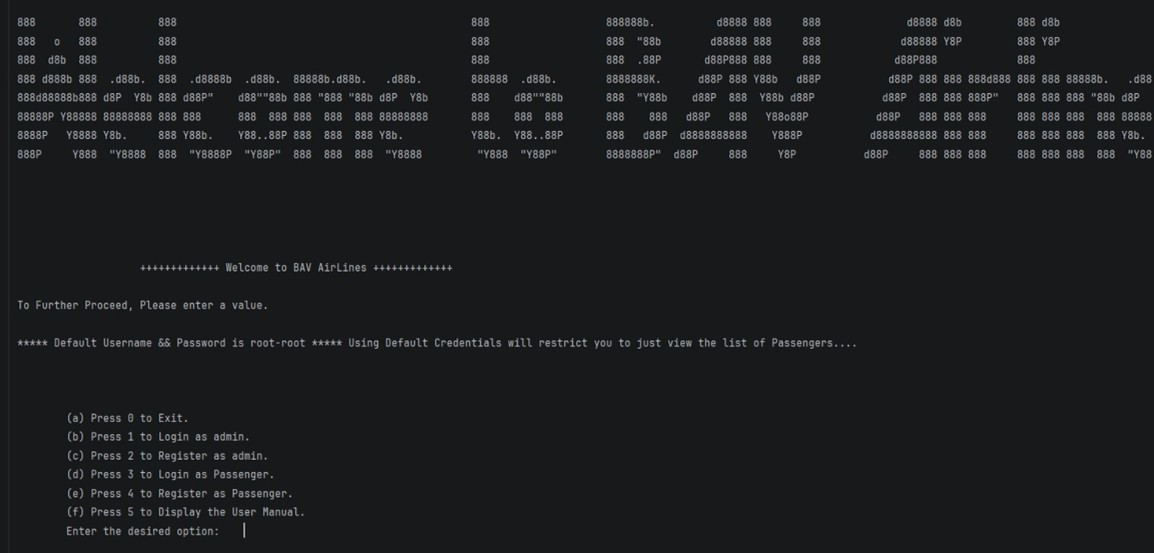
\includegraphics[width=\textwidth]{Figures/homepage.jpg}
\caption{Main Menu of Airline Reservation System}
\end{figure}
\vspace{-5pt}



As shown in Figure~5.1, the main menu provides options such as admin login, passenger login, registration, and access to the user manual. This menu ensures smooth navigation and improves user interaction with the system.

\FloatBarrier

\subsection{User Registration}

The user registration module enables new users to create an account by entering the required personal details.

\begin{figure}[H]
\centering
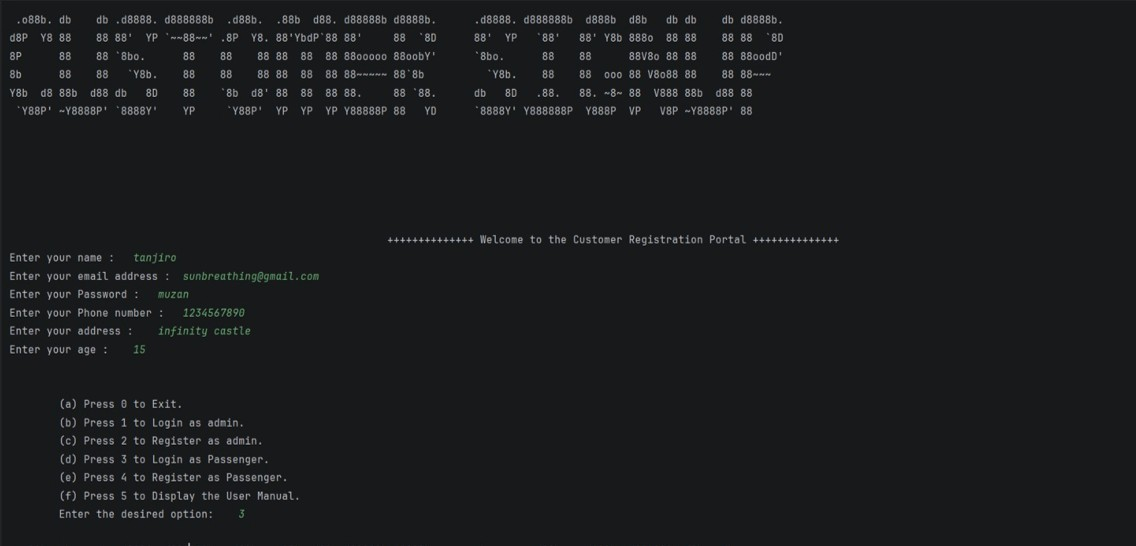
\includegraphics[width=\textwidth]{Figures/Picture2.jpg}
\caption{User Registration Interface}
\end{figure}
\vspace{-5pt}

As illustrated in Figure~5.2, the system collects essential user information such as name, email, password, phone number, and address. This module ensures secure and organized storage of user data for future login and booking operations.

\FloatBarrier

\section{Flight Management}

\subsection{Flight Schedule Display}

The flight schedule module provides users with detailed information about available flights.

\begin{figure}[H]
\centering
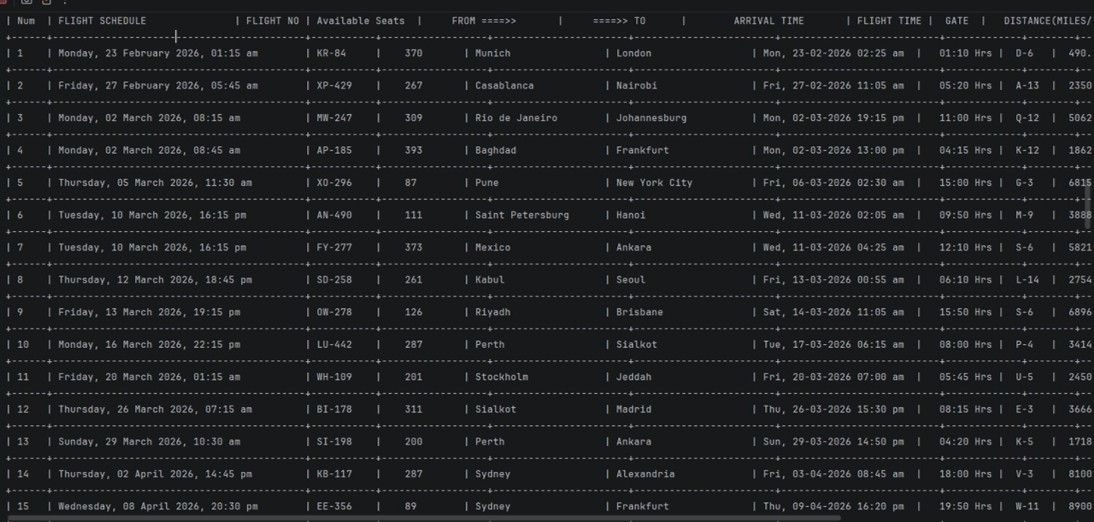
\includegraphics[width=\textwidth]{Figures/Picture4.jpg}
\caption{Flight Schedule Display}
\end{figure}
\vspace{-5pt}

Figure~5.3 shows the list of available flights along with important details such as flight number, available seats, departure location, destination, arrival time, and flight duration. This helps users make informed decisions while booking tickets.

\FloatBarrier

\subsection{Ticket Booking}

The ticket booking module allows users to reserve seats based on their preferences.

\begin{figure}[H]
\centering
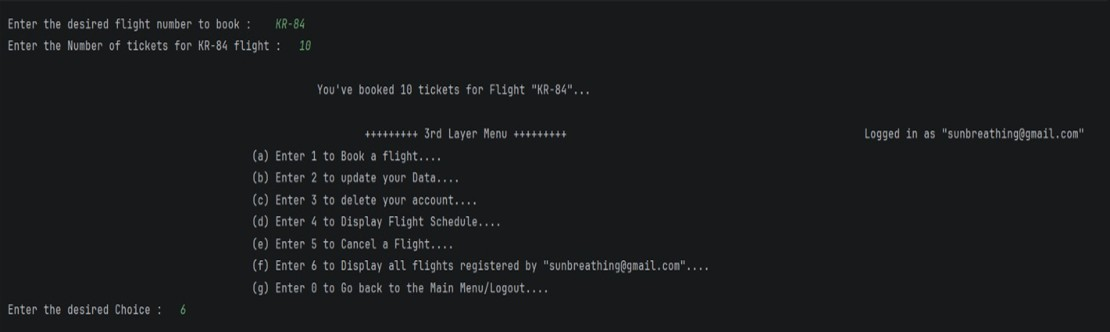
\includegraphics[width=\textwidth]{Figures/Picture5.jpg}
\caption{Ticket Booking Process}
\end{figure}
\vspace{-5pt}

As depicted in Figure~5.4, users can select a flight and enter the number of tickets required. The system processes the request and confirms the booking, ensuring real-time seat allocation and accuracy.

\FloatBarrier

\section{User Operations}

\subsection{User Menu Options}

After successful login, users are provided with multiple options to manage their activities within the system.

\begin{figure}[H]
\centering
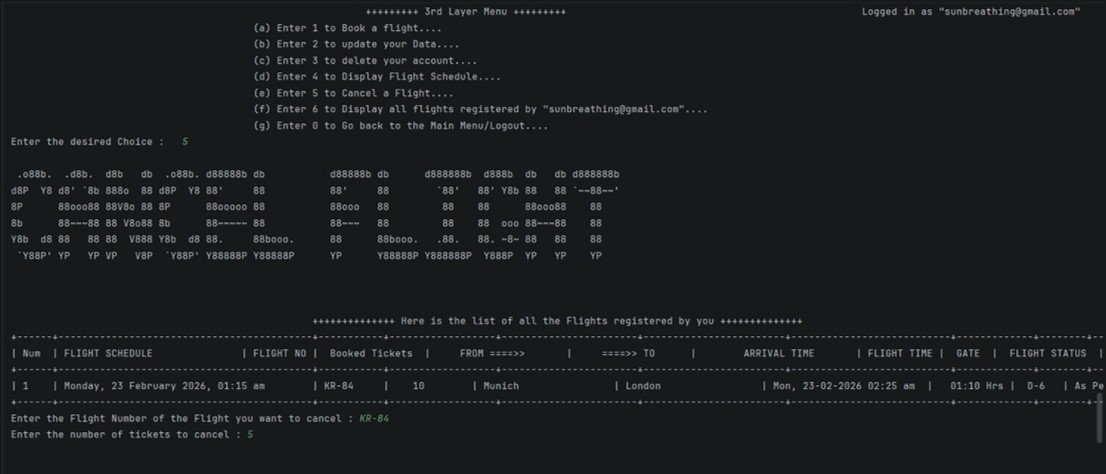
\includegraphics[width=\textwidth]{Figures/Picture7.jpg}
\caption{User Menu Interface}
\end{figure}
\vspace{-5pt}

Figure~5.5 illustrates the user menu, which includes options such as booking flights, updating personal details, viewing flight schedules, and canceling bookings. This enhances user control and flexibility.

\FloatBarrier

\subsection{Booking Details and Cancellation}

The system also provides functionality to view and manage booked tickets.

\begin{figure}[H]
\centering
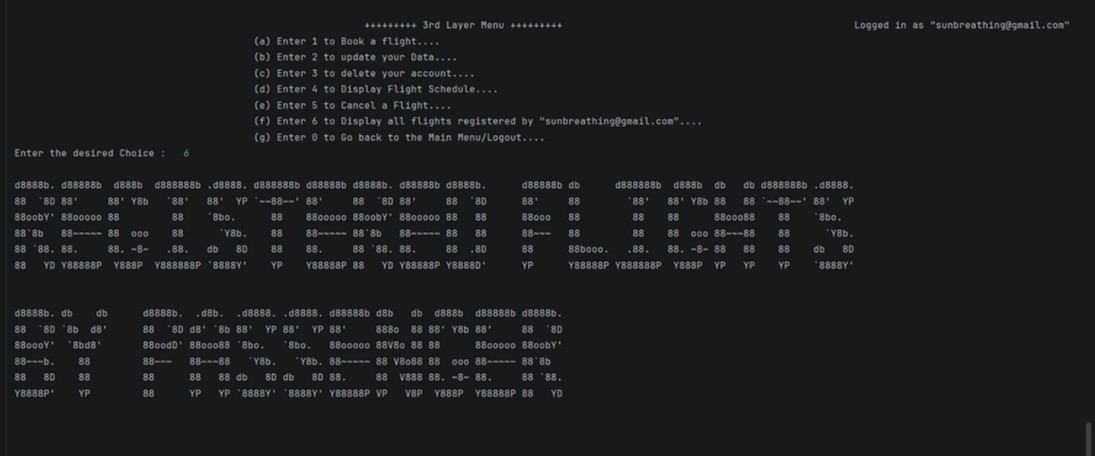
\includegraphics[width=\textwidth]{Figures/Picture8.jpg}
\caption{Booking Details and Cancellation}
\end{figure}
\vspace{-5pt}

As shown in Figure~5.6, users can view their booking details and cancel tickets if required. This feature ensures better management of reservations and improves overall user experience.
\bibitem{airline_uml}
\textbf{output :}
https://vscode.dev/github/recluzegeek/AirLineReservationSystem/blob/main
\FloatBarrier

\section{Summary}

This chapter demonstrated the implementation of the Airline Reservation System using various modules and console-based interfaces. The system effectively handles user interactions, flight management, and booking operations, ensuring accuracy, reliability, and ease of use.